\documentclass[english]{article}
\usepackage{comment}
\usepackage[letterpaper]{geometry}
\usepackage{tikz}
\usepackage{amsmath}
\usepackage{amsfonts}
\usepackage{amssymb}
\usepackage{float}
\usepackage{graphicx}
\usepackage{listings}
\usepackage{xcolor}

 
\definecolor{codegreen}{rgb}{0,0.6,0}
\definecolor{codegray}{rgb}{0.5,0.5,0.5}
\definecolor{codepurple}{rgb}{0.58,0,0.82}
\definecolor{backcolour}{rgb}{0.95,0.95,0.92}
 
\lstdefinestyle{mystyle}{
    backgroundcolor=\color{backcolour},   
    commentstyle=\color{codegreen},
    keywordstyle=\color{magenta},
    numberstyle=\tiny\color{codegray},
    stringstyle=\color{codepurple},
    basicstyle=\ttfamily\footnotesize,
    breakatwhitespace=false,         
    breaklines=true,                 
    captionpos=b,                    
    keepspaces=true,                 
    numbers=left,                    
    numbersep=5pt,                  
    showspaces=false,                
    showstringspaces=false,
    showtabs=false,                  
    tabsize=2
}
 
\lstset{style=mystyle}


\geometry{verbose,tmargin=1in,bmargin=1in,lmargin=1in,rmargin=1in}

\renewcommand{\u}{{\mathbf u}}
\newcommand{\x}{{\mathbf x}}
\newcommand{\R}{{\mathbb R}}


\title{CIS 520, Machine Learning, Fall 2020 \\ Homework 6\\
Due: Monday, November 9th, 11:59pm \\
Submit to Gradescope}
\date{}
\author{Yuezhong Chen, Sheil Sarda}


\begin{document}
\maketitle
\section{Programming: Missing Data Imputation}
For this question, refer to the Jupyter Notebook. You will be implementing different imputation techniques -- the notebook will have detailed instructions.

\subsection{Zero Imputation}
Look for the code marked \verb|#TODO| in the notebook and complete the code between the segments according to the instructions. \\

\begin{itemize}
    \item 
Add the accuracy and the Frobenius norm in this report.

\begin{table}[H]
\centering
\begin{tabular}{ |c|c| } 
 \hline
 Frobenius Norm & 51.668 \\
 Accuracy & 60.0\% \\
 \hline
\end{tabular}
\caption{Accuracy and Frobenius norm for Zero Imputation}
\label{nnOA}
\end{table}

\item
Add the code of the completed zeroImpute method. 
\begin{lstlisting}[language = Python, caption=zeroImpute method]
def zeroImpute(X_miss):
  '''
  Returns :
  X_imputed which has zeroes instead of missing values and same shape as X_miss.
  '''
  X_imputed = X_miss.copy()

  # replace missing values with zeroes
  X_imputed = np.nan_to_num(X_imputed)

  assert X_imputed.shape == X_miss.shape

  return X_imputed
\end{lstlisting}


\end{itemize}


\subsection{Mean Imputation}
Look for the code marked \verb|#TODO| in the notebook and complete the code between the segments according to the instructions. \\

\begin{itemize}
    \item 
Add the accuracy and the Frobenius norm in this report.

\begin{table}[H]
\centering
\begin{tabular}{ |c|c|c| } 
 \hline
 Frobenius Norm & 13.7633 \\
 Accuracy & 84.0\% \\
 \hline
\end{tabular}
\caption{Accuracy and Frobenius norm for Mean Imputation}
\label{nnOA}
\end{table}


\item
Add the code of the completed meanImpute method. 
\begin{lstlisting}[language = Python, caption=meanImpute method]
def meanImpute(X_miss):
  '''
  Returns :
  X_imputed which has mean of the corresponding column instead of the missing values and same shape as X_miss.
  '''
  X_imputed = X_miss.copy()

  # replace the value of NaNs with the mean of their column.
  X_imputed = np.apply_along_axis(lambda val: 
                                  np.nan_to_num(val, nan=np.nanmean(val)),
                                  0, X_imputed) 

  assert X_imputed.shape == X_miss.shape

  return X_imputed
\end{lstlisting}

\end{itemize}

\subsection{Regression Imputation}
Look for the code marked \verb|#TODO| in the notebook and complete the code between the segments according to the instructions. \\

\begin{itemize}
    \item 
Complete the following table.



\begin{table}[H]
\centering
\begin{tabular}{ |c|c|c| } 
 \hline
 \textbf{Epoch} & \textbf{Frobenius Norm} & \textbf{Accuracy} \\
 \hline
 After Base Imputation & 51.668 & 60.0\% \\
 1 & 23.930 & 74.0\% \\
 2 & 13.986 & 84.0\% \\
 3 & 11.394 & 86.0\% \\
 4 & 10.490 & 90.0\% \\
 5 & 10.047 & 92.0\% \\
 \hline
\end{tabular}
\caption{Accuracy and Frobenius norm for Zero Imputation}
\label{nnOA}
\end{table}


\item Plot for Accuracy for Regression based imputation vs. Number of Features imputed\\
    \begin{figure}[H]
    	\centering
    	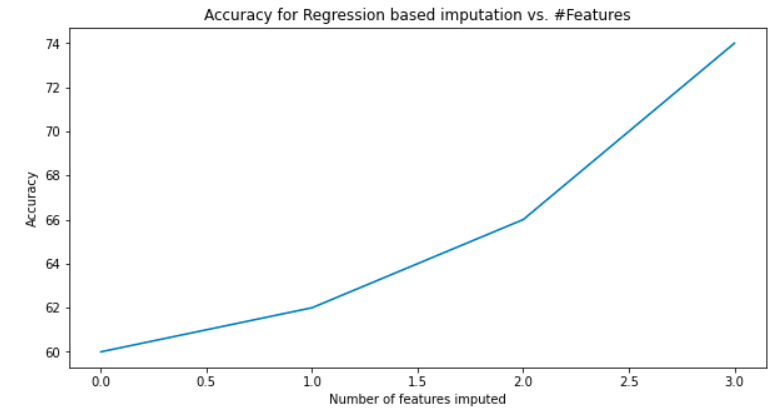
\includegraphics[width=.7\textwidth]{templates/accuracy_vs_features}
    	\label{fig:my_label}
    \end{figure}

\item Plot for Norm for Regression based imputation vs. Number of Features imputed\\
    \begin{figure}[H]
    	\centering
    	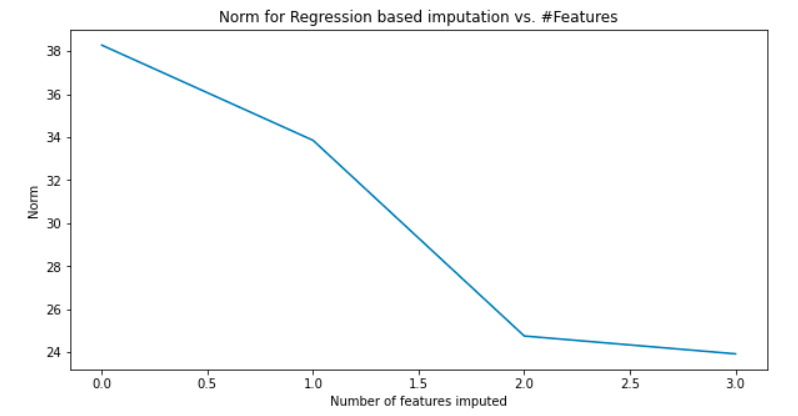
\includegraphics[width=.7\textwidth]{templates/norm_vs_features}
    	\label{fig:my_label}
    \end{figure}

\item Plot for Accuracy for Regression based imputation vs Number of Epochs\\
    \begin{figure}[H]
    	\centering
    	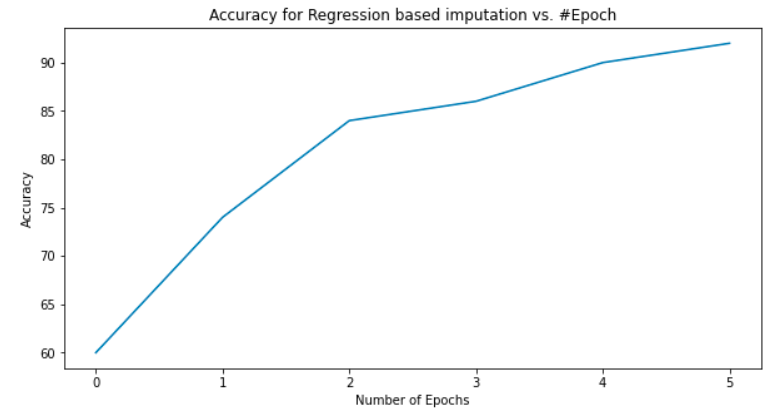
\includegraphics[width=.7\textwidth]{templates/accuracy_vs_epoch}
    	\label{fig:my_label}
    \end{figure}

\item Plot for Norm for Regression based imputation vs. Number of Epochs\\
    \begin{figure}[H]
    	\centering
    	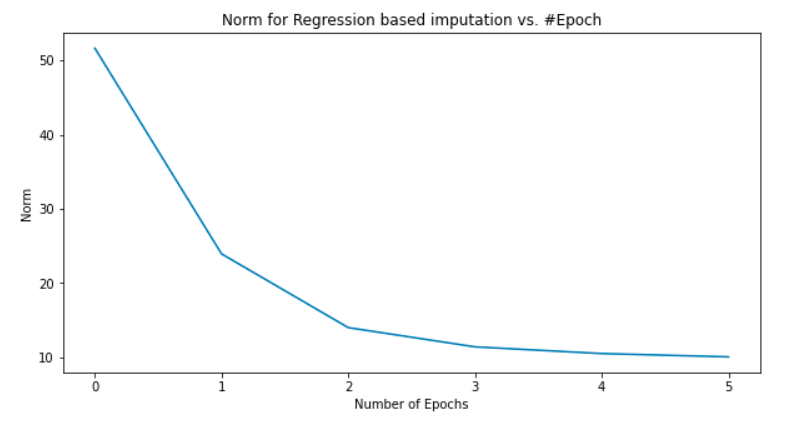
\includegraphics[width=.7\textwidth]{templates/norm_vs_epoch}
    	\label{fig:my_label}
    \end{figure}

\item
Add the code of the completed regressedImpute method. 
\begin{lstlisting}[language = Python, caption=regressedImpute method]
def regressedImpute(X_baseImputed, X_miss, 
                    X_test, y_test, computePerFeatureStatistics = False):
    '''
    Returns :
    X_imputed which has mean of the linearly regressed value instead of the 
    missing values and same shape as X_miss.

    if computePerFeatureStatistics is True, also:
    list of Frobenius norms of difference between reconstructions and original data 
    (without missing values) calculated after each imputing each column.
    list of accuracies on test set of Logistic Regression classifier trained 
    on imputed data after each imputing each column.
    '''
    X_imputed = X_baseImputed.copy()
    frobenius_norms =[]
    accuracies =[]
    
    # We do a linear regression based imputation here, for each column, train a 
    # classifier to predict its value based on values of other features and
    # replace the NaN with the predicted values. 
    # IMPORTANT : You should not use regressed values from an earlier column to predict 
    #             a later column, make sure to train the regression model on base 
    #             imputed and not modify base imputed during the run.
    #             You can use X_miss to find which values were originally NaNs.
    
    for i in range(X_baseImputed.shape[1]):
        
        nan_ix = np.isnan(X_miss[:, i])
        x_train = np.delete(X_baseImputed, i, axis=1)
        y_train = X_baseImputed[:, i]
        
        m = LinearRegression()
        m.fit(x_train, y_train)
        pred = m.predict(x_train)
        
        X_imputed[nan_ix, i] = pred[nan_ix]

        if computePerFeatureStatistics == True:
            clf = LogisticRegression()
            clf.fit(X_imputed, y_miss)
            accuracies.append(clf.score(X_test, y_test))
            frobenius_norms.append(LA.norm(X_train - X_imputed))
            

    if computePerFeatureStatistics == True:
        return X_imputed, frobenius_norms, accuracies
    else:
        return X_imputed
\end{lstlisting}
\end{itemize}


\subsection{Follow Up Questions}
\begin{enumerate}

    
    \item  Which is the best of the three imputation methods? Why (briefly)?
    	\newline \newline
    	The Linear Regression imputation technique is the best of the three considered above since it yields the highest accuracy and smallest Frobenius norm in the test set.
     
      \item Could you potentially do a better job of imputation if you also used y vales as well as x's? How might that help? If using the y's for imputation helps, why do people mostly not use them?
      \newline
      \newline
      To answer the last question, $Y$ is generally  not used to predict $X$ because this can very quickly lead to over-fitting, since when we try to generalize this model and run it on the test set, we will not have access to the test labels by design. 
      \newline
      \newline
      Generally, $Y$ is correlated with $X$, so using the labels to impute missing inputs can lead to better performance. However, due to the above considerations, this is not a good strategy.
         
    \item Describe the trend for the accuracy and the norm as impute more features for regression imputation. Give a plausible explanation behind the trend.
    \newline
    \newline
	The general trend as we impute more features for regression is that the Frobenius norm decreases and the accuracy of our imputations increases.
    \newline
    \newline
    As we impute more features, we learn more about the original distribution used to create $X$. This added information about the latent distribution makes our norm shrink and the predictive power of $Y$ increase.    
    \item Describe the trend for the accuracy and the norm as re-impute again for several epochs for regression imputation. Give a plausible explanation behind the trend.
        \newline
        \newline
    	The general trend as we re-impute features for several epochs in the regression is that the Frobenius norm decreases and the accuracy of our imputations increases.
        \newline
        \newline
	This is caused by the fact that with each epoch, the regressor uses the past approximation of $X$ to generate the next one, causing the approximation to improve with each epoch.    
    
\end{enumerate}
\section{Programming: K-Means Analysis}
In this assignment, we will implement the K-means algorithm and perform it on a breast cancer data set. Please follow the attached Python notebook to write and plot the functions.
\subsection{Part 1: K-means iteration function}
Write the K-means iteration function as is described in the notebook. Each iteration takes the data and current centroid values for each class as parameters, and returns both updated centroid values along with a list of labels telling which class each datapoint belongs to.
\begin{enumerate}
    \item  Fill in the table below by reporting the resulting cluster labels and resulting centroids from running the iteration function on the given parameters.
            \begin{center}
            \begin{tabular}{|c|c|c|c|}
                \hline
                \textbf{X} & \textbf{Initial Centroids} & \textbf{Resulting Cluster Labels} & \textbf{Resulting Centroids}  \\
                 \hline
                [[1], [2], [10], [12]]  & [1, 2] & \verb|[0, 1, 1, 1]|& \verb|[[1.0], [8.0]]|  \\ \hline
                [[1], [2], [10], [12]]  & [1, 8] & \verb|[0, 0, 1, 1]| & \verb|[[1.5], [11.0]]| \\ \hline
               [[1], [2], [10], [12]]  & [2, 2] & \verb|[0, 0, 0, 0]| & \verb|[[6.25], [2.0]]|  \\ \hline
                [[0,5,0],[0,5,0],[0,4,3],[0,3,4]] & [[2.5,0,0],[-2.5,0,0]] & \verb|[0, 0, 0, 0]| & [[0.0, 4.25, 1.75], [-2.5, 0.0, 0.0]]  \\ \hline
                
            \end{tabular}
            \end{center}
        
    \item 
    If an iteration of the k-means algorithm returns less than K classes, what might that indicate about the data?
	\newline
	\newline
	This might indicate that $K$ classes is too many, and that fewer classes would suffice.

\end{enumerate}


\subsection{Part 2: Putting the algorithm together}
Now write the whole K-means function using your iteration function, as is described in the notebook. The function takes in the data set with the number of classes and returns the final centroid values, the final list of labels telling which class each data point belongs to, and the number of K-means iterations.
\begin{enumerate}
    \item Put your 3 sanity-check graphs here.
\begin{figure}[H]
    	\centering
    	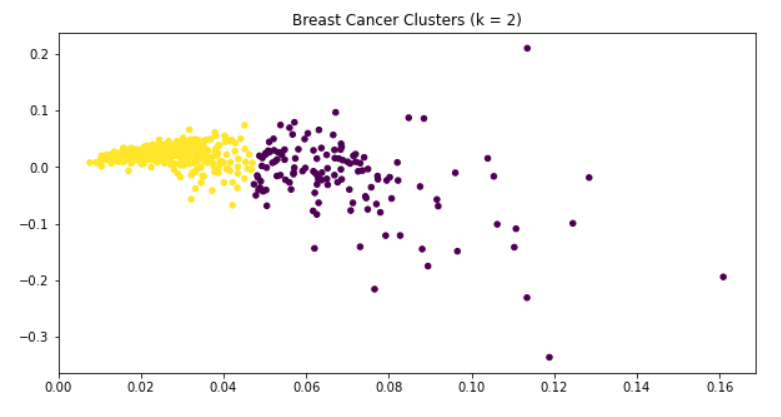
\includegraphics[width=.7\textwidth]{templates/k2}
    	\label{fig:my_label}
    \end{figure}
\begin{figure}[H]
    	\centering
    	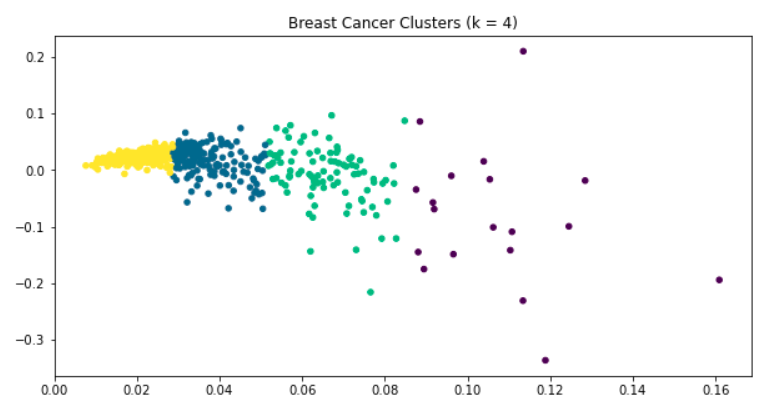
\includegraphics[width=.7\textwidth]{templates/k4}
    	\label{fig:my_label}
    \end{figure}
\begin{figure}[H]
    	\centering
    	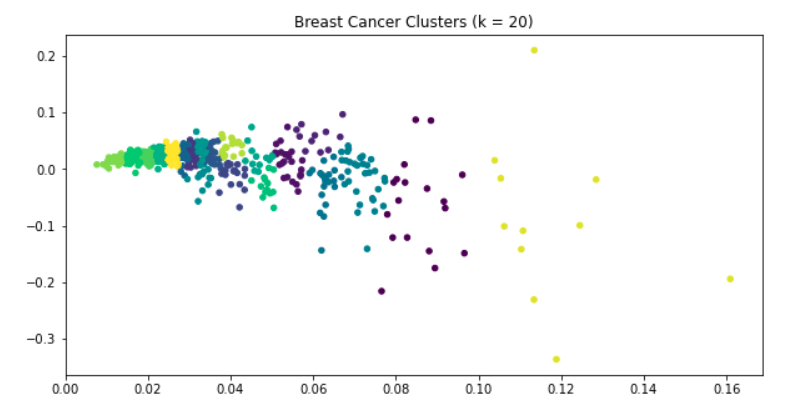
\includegraphics[width=.7\textwidth]{templates/k20}
    	\label{fig:my_label}
    \end{figure}
    
    \item Write down how many iterations it took for your k-means to converge for each of the sanity-check graphs. How does this number compare with what you expected it to be? How does the number of iterations seem to vary proportional to k?
    \begin{itemize}
\item $k = 2$ took 8 iterations.
\item $k = 4$ took 22 iterations.
\item $k = 20$ took 19 iterations.
    \end{itemize}

        The number of iterations seems to be positively correlated with $k$ for $k < 10$ but this relationship seems to break down for large $k$ such as $k = 20$. This indicates that convergence speeds up for large $k$ because the number of points in each class decreases as $k$ increases.
\end{enumerate}
\subsection{Part 3: Choosing the value of K}
Write the test$\_$cluster$\_$size function using your k-means function, as is described in the notebook. The function takes in the data set with the number of classes and returns a list of scores where each score is the distortion for that value of k.
\begin{enumerate}
    \item Using the breast cancer data set, record your labeled plots for distortion, min-max scaled distortion, and log scaled distortion here
    \newline
    \begin{figure}[H]
        	\centering
        	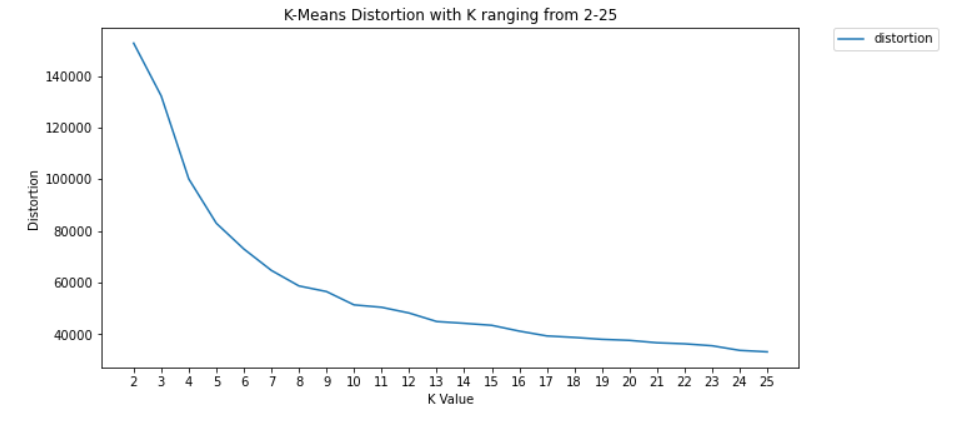
\includegraphics[width=.7\textwidth]{templates/distortion}
        	\label{fig:my_label}
        \end{figure}
\begin{figure}[H]
    	\centering
    	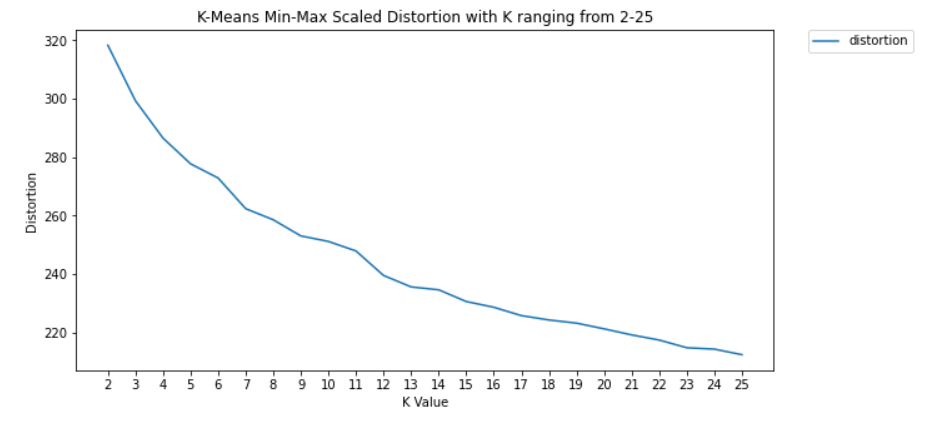
\includegraphics[width=.7\textwidth]{templates/scaled_distortion}
    	\label{fig:my_label}
    \end{figure}
\begin{figure}[H]
    	\centering
    	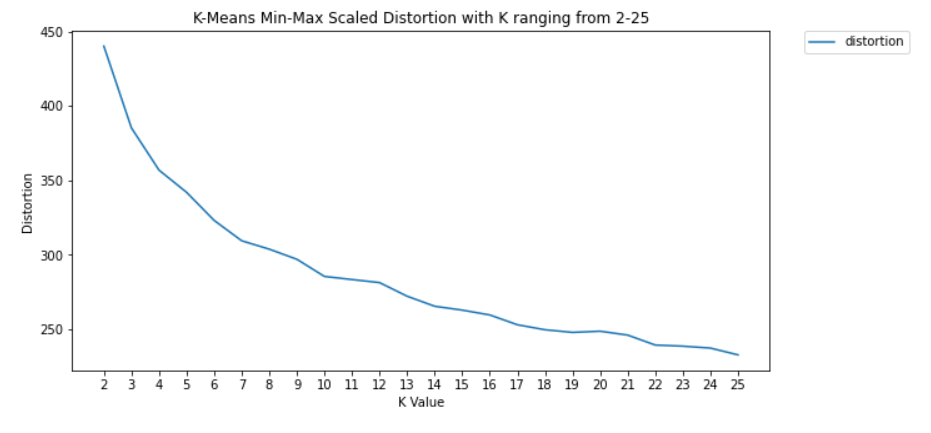
\includegraphics[width=.7\textwidth]{templates/minmax_distortion}
    	\label{fig:my_label}
    \end{figure}            
    \item Why can't we hold out some of the data in a validation set, and choose the value of k which minimizes a cross-validation error like we have in the past for algorithms like linear regression?
    \newline
    \newline
    We were able to hold out some of the data in a validation set when performing linear regression because it is a supervised learning problem. In this case, we are not able to do this because this is an unsupervised learning problem where there is no validation error we are trying to minimize.
\end{enumerate}

\section{Performance Measures for Face Detection in Images}
Consider a face detection problem, where the goal is to build a system that can automatically detect faces in images. Two research groups develop systems for this problem using slightly different approaches. In both cases, the central component of the system is a binary classifier which, when applied to a $24 \times 24$ image, decides whether or not it is a face. The two groups train their classifiers using different learning algorithms. Moreover, when given a new image, they also apply their classifiers in slightly different ways: group A tests $24 \times 24$ regions of the image taking strides of size 2 (so, for example, for a $100 \times 100$ image, $(39)^2$ regions would be tested); group B tests $24 \times 24$ regions of the image taking strides of size 5 (so here, for a $100 \times 100$ image, only $(16)^2$ regions would be tested).\footnote{In practice, the $24\times 24$ classifier would also be applied to multiple scaled versions of the input image; we ignore this issue here for simplicity.}
On a standard benchmark suite of test images that contains 300 faces altogether, the two groups have the following performances (assume the regions tested by both systems include all the 300 true face regions):

\begin{center}
\begin{tabular}{|c|c|c|c|}
\hline
\textbf{Research group} & \textbf{Number of regions} & \textbf{Number of faces} & \textbf{Number of non-face regions} \\
	& \textbf{tested} & \textbf{detected correctly} & \textbf{detected as faces} \\
\hline
A & 20,000 & 280 & 100 \\
\hline
B & 12,500 & 270 & 60 \\
\hline
\end{tabular}
\end{center}

\begin{enumerate}
\item 
Based on the above numbers, calculate the TPR (recall), TNR, and precision of each group's system as tested. 
Also calculate the resulting geometric mean (GM) and $F_1$ measures for each system.
If you were to select a system based on the GM measure, which system would you choose? Would your choice change if you were to select a system based on the $F_1$ measure? (Note, the geometric mean (GM) is defined as $\sqrt{TPR\times TNR}$.)

Research Group A:
    TPR = 0.9333, TNR = 0.9949, precision = 0.7368\\
Research Group B:
    TPR = 0.9000, TNR = 0.9951, precision = 0.8182\\
And for Group A: GM = 0.9636, F1 = 0.8235\\
And for Group B: GM = 0.9462, F1 = 0.8571\\
   
For GM measure we select A, and we will change to B based on the F1 measure.\\
    
\item 
Which performance measure would be more suitable for this problem -- the GM measure or the $F_1$ measure? Why?

$F_1$ measure. 

Comparing to $F_1$, GM measure releases more information about recognizing non-face regions as faces. In this regard, $F_1$ is more suitable.\\
    
\item  Another way to determine which method to choose would be to look at the ROC curve. Because you are given instances of different algorithms, not the algorithm itself, each method corresponds to a \textit{point} on the TPR vs. FPR graph, not a curve. \\ \ \\ What is the Euclidean distance from each instance to the 0-error (perfect classification) point $(0,1)$? Based on this metric, which method would you choose? 

A: 0.0669, B:0.1001\\
A will be chosen, because it is closer to the perfect point.

\item 
Now assume that there is a third group C which trains their classifier using a newly discovered learning algorithm. Some of the resulting statistical measures are described below:

\begin{center}
\begin{tabular}{|c|c|c|c|c|}

\hline
\textbf{Research group} & \textbf{TPR} & \textbf{TNR} & \textbf{FPR} & \textbf{FNR}  \\
\hline 
C & 0.95 & 0.990 & 0.01 & 0.05 \\
\hline

\end{tabular}
\end{center}

\begin{enumerate}
    \item Suppose you worked for a social media platform, where you want to identify as many faces as possible for your photo tagging systems (prioritize recall). Would you prefer the algorithm created by group C over the algorithms created by groups A and B?\\
    
    Yes. Because the TPR of A and B are smaller than that of C in this case.
    
    \item Now suppose you worked for law enforcement, where every face detected will be checked against a criminal database, which is an expensive operation. You'd like maximize specificity (1 - FPR) in this case to avoid unnecessary costs. Would you prefer the algorithm created by group C over the algorithms created by groups A and B?\\
    
    No. Because the TPR of A and B are larger than that of C in this case.
    
\end{enumerate}


\end{enumerate}
\section{EM Algorithm with Red and Blue Coins} 
Your friend has two coins: a red coin and a blue coin, with biases $p_r$ and $p_b$, respectively (i.e.\ the red coin comes up heads with probability $p_r$, and the blue coin does so with probability $p_b$). She also has an inherent preference $\pi$ for the red coin. She conducts a sequence of $m$ coin tosses: for each toss, she first picks either the red coin with probability $\pi$ or the blue coin with probability $1-\pi$, and then tosses the corresponding coin; the process for each toss is carried out independently of all other tosses. 
You don't know which coin was used on each toss; all you are told are the outcomes of the $m$ tosses (heads or tails). In particular, for each toss $i$, define a random variable $X_i$ as 
\[
X_i = \begin{cases}
	1 & ~~\text{if the $i$-th toss results in heads} \\
	0 & ~~\text{otherwise.}
	\end{cases}
\] 
Then the data you see are the values $x_1,\ldots,x_m$ taken by these $m$ random variables.
Based on this data, you want to estimate the parameters $\theta = (\pi, p_r, p_b)$.
To help with this, for each toss $i$, define a latent (unobserved) random variable $Z_i$ as follows:
\[
Z_i = \begin{cases}
	1 & ~~\text{if the $i$-th toss used the red coin} \\
	0 & ~~\text{otherwise.}
	\end{cases}
\]

\begin{enumerate}
\item
Let $X$ be a random variable denoting the outcome of a coin toss according to the process described above, and let $Z$ be the corresponding latent random variable indicating which coin was used, also as described above (both $X$ and $Z$ take values in $\{0,1\}$ as above).
Write an expression for the joint distribution of $X$ and $Z$.
Give your answer in the form 
\[
p(x,z; \, \theta) = \rule{5cm}{0.5pt}
	\,.
\]

Solution:\\
Through the conditional probability property, we have: $p(x,z; \, \theta) = p(x|z,\theta) p(z|\theta)$, then

$p(x|z,\theta) p(z|\theta)= (p_r^x(1-p_r)^{1-x})^{z}(p_b^x(1-p_b)^{1-x})^{1-z}(\pi^z(1-\pi)^{1-z})$\\ $= (\pi p_r^x(1-p_r)^{1-x})^{z}((1-\pi)p_b^x(1-p_b)^{1-x})^{1-z}$\\
Thus, $p(x,z; \, \theta)= (\pi p_r^x(1-p_r)^{1-x})^{z}((1-\pi)p_b^x(1-p_b)^{1-x})^{1-z}$\\


\item 
Write an expression for the complete-data log-likelihood, \\

From question 1, we know \\
$ln \L_c(\theta) = \sum_{i=1}^m ln p(x_i,z_i; \, \theta) = \sum_{i=1}^{m}[z_iln(\pi p_r^{x_i}(1-p_r)^{1-x_i})+(1-z_i)ln((1-\pi)p_b^{x_i}(1-p_b)^{1-x_i})
    ]=\sum_{i=1}^{m}[z_i(ln(\pi)+x_iln(p_r)+(1-x_i)ln(1-p_r))+(1-z_i)(ln(1-\pi)+x_iln(p_b)+(1-x_i)ln(1-p_b))]$\\

\item 
Suppose you knew the values $z_i$ taken by the latent variables $Z_i$. What would be the maximum-likelihood parameter estimates $\hat{\theta}$? Give expressions for $\hat{\pi}$, $\hat{p}_r$, and $\hat{p}_b$ (in terms of $x_i$ and $z_i$).

$ \hat{\pi} = \frac{\sum_{i=1}^{m}z_i}{m},
 \hat{p}_r = \frac{\sum_{i=1}^{m}z_ix_i}{\sum_{i=1}^{m}z_i},
 \hat{p}_b = \frac{\sum_{i=1}^{m}(1-z_i)x_i}{\sum_{i=1}^{m}(1-z_i)} $

\item
In the absence of knowledge of $z_i$, one possibility for estimating $\theta$ is to use the EM algorithm. Recall that the algorithm starts with some initial parameter estimates $\theta^0$, and then on each iteration $t$, performs an E-step followed by an M-step. Let $\theta^t$ denote the parameter estimates at the start of iteration $t$. In the E-step, for each toss $i$, the algorithm requires computing the posterior distribution of the latent variable $Z_i$ under the current parameters $\theta^t$. Calculate the posterior probability $\P(Z_i = 1 \,|\, X_i = x_i; \,\theta^t)$. 
\emph{(Hint: Use Bayes' rule.)}

By using the Bayes' Rule, we have:\\
\[
P(Z_i = 1 \,|\, X_i = x_i; \,\theta^t) = \frac{P(X_i=x_i|Z_i=1)P(Z_i=1)}{\sum_{a=0,1}P(X_i=x_i|Z_i=a)P(Z_i=a)}
= \frac{p_{rt}^{x_i}(1-p_{rt})^{1-x_i}\pi_t}{(p_{bt}^{x_i}(1-p_{bt})^{1-x_i})(1-\pi_t)+p_{rt}^{x_i}(1-p_{rt})^{1-x_i}\pi_t}
\]

\item 
For each toss $i$, denote the posterior probability computed in part (d) above by $\gamma^{t}_i$ (so that $\gamma^{t}_i = P(Z_i = 1 \,|\, X_i = x_i; \, \theta^t)$).
Then the expected complete-data log-likelihood with respect to these posterior distributions is 
\[
%\E_{Z_1,\ldots,Z_m}[\, \ln \L_c(\theta) \,] = 
\sum_{i=1}^m \Big( \gamma^{t}_i \cdot \ln p(x_i,1; \, \theta) + (1-\gamma^{t}_i) \cdot \ln p(x_i,0; \, \theta) \Big)
	\,.
\]
The M-step of the EM algorithm requires finding parameters $\theta^{t+1}$ that maximize this expected complete-data log-likelihood.

Determine the updated parameters $\theta^{t+1}$. Give expressions for $\pi^{t+1}$, $p_r^{t+1}$, and $p_b^{t+1}$ (in terms of $x_i$ and $\gamma^{t}_i$).

\[
\hat{\pi}^{t+1} = \frac{\sum_{i=1}^{m}\gamma_i^t}{m}, 
\hat{p}_r^{t+1} = \frac{\sum_{i=1}^{m}\gamma_i^tx_i}{\sum_{i=1}^{m}\gamma_i}, 
\hat{p}_b^{t+1} = \frac{\sum_{i=1}^{m}(1-\gamma_i^t)x_i}{\sum_{i=1}^{m}(1-\gamma_i^t)} 
\]
\end{enumerate}


\end{document}